\documentclass[border=12pt]{standalone}
\usepackage{tikz}
\usepackage{helvet}
\usepackage{amsmath,amssymb}
\renewcommand{\familydefault}{\sfdefault}
\usetikzlibrary{arrows.meta, positioning, calc, shapes.geometric, shapes.symbols, fit, backgrounds, patterns}

\definecolor{emeraldpine}{HTML}{1A4D3E}
\definecolor{harvardcrimson}{HTML}{A51C30}
\definecolor{ethdarkblue}{HTML}{1F407A}
\definecolor{ethpetrol}{HTML}{007A87}
\definecolor{ethbronze}{HTML}{B87333}
\definecolor{ink}{HTML}{1A202C}
\definecolor{softink}{HTML}{4A5568}
\definecolor{paleink}{HTML}{94A3B8}
\definecolor{cardbg}{HTML}{F8FAFC}
\definecolor{shadecolor}{HTML}{F1F5F9}
\definecolor{faultbg}{HTML}{FFF1F2}
\definecolor{safeaccent}{HTML}{E6F4EA}
\definecolor{faultaccent}{HTML}{FEE2E2}

\tikzset{
    box/.style={draw, rounded corners=3pt, align=center, font=\footnotesize, thick, fill=white},
    boxA/.style={box, draw=emeraldpine, minimum width=2.0cm, minimum height=1.1cm},
    boxB/.style={box, draw=softink, text=ink, minimum width=2.0cm, minimum height=1.1cm},
    loadA/.style={box, draw=emeraldpine, fill=emeraldpine!12, minimum width=2.5cm, minimum height=1.1cm},
    loadB/.style={box, draw=softink, fill=white, minimum width=2.5cm, minimum height=1.1cm},
    railA/.style={draw=emeraldpine, line width=1.5pt},
    railB_healthy/.style={draw=ethdarkblue, line width=1.5pt},
    railB_tripped/.style={draw=harvardcrimson, dashed, line width=1.2pt}
}

\begin{document}
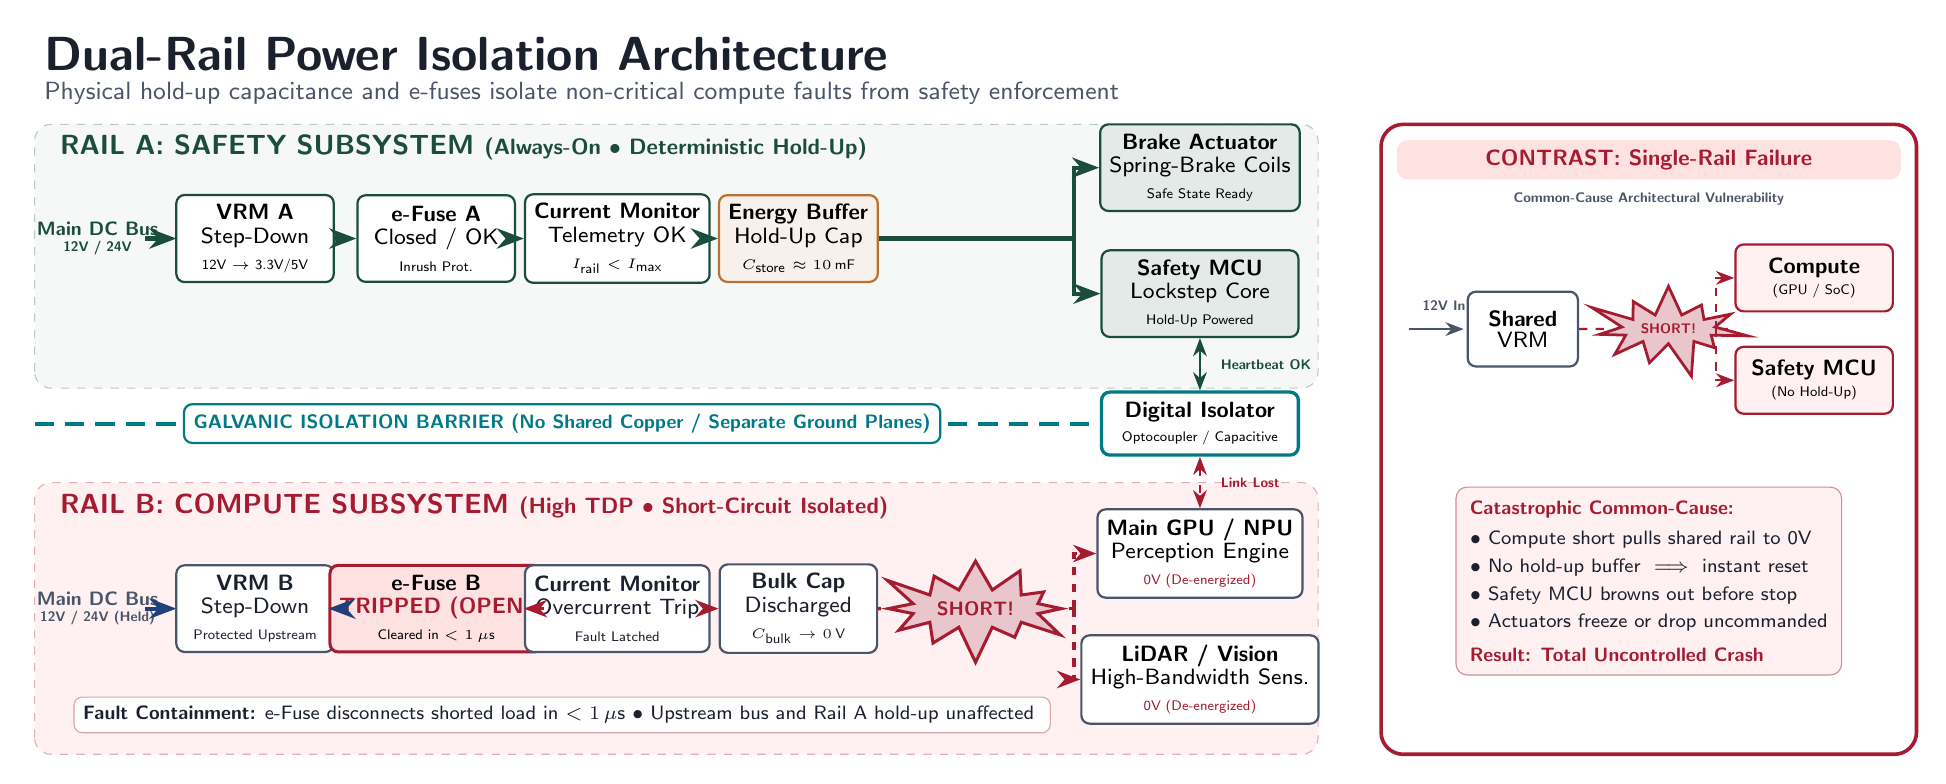
\begin{tikzpicture}[>=Stealth, font=\sffamily]

% Title and Subtitle
\node[anchor=west, font=\LARGE\bfseries, text=ink] at (-1.0, 4.70) {Dual-Rail Power Isolation Architecture};
\node[anchor=west, font=\small, text=softink] at (-1.0, 4.20) {Physical hold-up capacitance and e-fuses isolate non-critical compute faults from safety enforcement};

% ==================== RAIL A (SAFETY) ====================
% Background Card
\fill[emeraldpine!4, rounded corners=6pt] (-1.0, 0.45) rectangle (15.3, 3.80);
\draw[emeraldpine!30, dashed, rounded corners=6pt] (-1.0, 0.45) rectangle (15.3, 3.80);

% Section Header
\node[font=\bfseries, text=emeraldpine, anchor=west] at (-0.8, 3.50) {RAIL A: SAFETY SUBSYSTEM \footnotesize (Always-On $\bullet$ Deterministic Hold-Up)};

% Input Power
\node[font=\scriptsize\bfseries, text=emeraldpine, align=center] at (-0.2, 2.35) {Main DC Bus\\[-2pt]{\tiny 12V / 24V}};
\draw[railA, ->] (0.4, 2.35) -- (0.8, 2.35);

% Rail A Components
\node[boxA] (vrmA) at (1.8, 2.35) {\textbf{VRM A}\\[-1pt]\footnotesize Step-Down\\\tiny 12V $\to$ 3.3V/5V};
\node[boxA] (fuseA) at (4.1, 2.35) {\textbf{e-Fuse A}\\[-1pt]\footnotesize Closed / OK\\\tiny Inrush Prot.};
\node[boxA] (monA) at (6.4, 2.35) {\textbf{Current Monitor}\\[-1pt]\footnotesize Telemetry OK\\\tiny $I_{\text{rail}} < I_{\text{max}}$};
\node[boxA, fill=ethbronze!10, draw=ethbronze] (capA) at (8.7, 2.35) {\textbf{Energy Buffer}\\[-1pt]\footnotesize Hold-Up Cap\\\tiny $C_{\text{store}} \approx 10\,\text{mF}$};

% Rail A Loads
\node[loadA] (actA) at (13.8, 3.25) {\textbf{Brake Actuator}\\[-1pt]\footnotesize Spring-Brake Coils\\\tiny Safe State Ready};
\node[loadA] (mcuA) at (13.8, 1.65) {\textbf{Safety MCU}\\[-1pt]\footnotesize Lockstep Core\\\tiny Hold-Up Powered};

% Rail A Interconnections
\draw[railA, ->] (vrmA) -- (fuseA);
\draw[railA, ->] (fuseA) -- (monA);
\draw[railA, ->] (monA) -- (capA);
\draw[railA] (capA.east) -- (12.2, 2.35);
\draw[railA, ->] (12.2, 2.35) |- (actA.west);
\draw[railA, ->] (12.2, 2.35) |- (mcuA.west);


% ==================== GALVANIC ISOLATION BARRIER ====================
% Digital Isolator
\node[box, draw=ethpetrol, fill=white, minimum width=2.5cm, minimum height=0.8cm, line width=1.2pt] (iso) at (13.8, 0.0) {\textbf{Digital Isolator}\\[-1pt]\tiny Optocoupler / Capacitive};

% Barrier line ends precisely at the isolator
\draw[line width=1.4pt, dash pattern=on 7pt off 4pt, ethpetrol] (-1.0, 0.0) -- (iso.west);
\node[fill=white, draw=ethpetrol, line width=0.8pt, rounded corners=3pt, font=\scriptsize\bfseries, text=ethpetrol, inner sep=3.5pt] at (5.7, 0.0) {GALVANIC ISOLATION BARRIER (No Shared Copper / Separate Ground Planes)};

\draw[thick, emeraldpine, <->] (mcuA.south) -- (iso.north);
\node[font=\tiny\bfseries, text=emeraldpine, right=4pt] at ($(mcuA.south)!0.5!(iso.north)$) {Heartbeat OK};


% ==================== RAIL B (COMPUTE) ====================
% Background Card
\fill[faultbg, rounded corners=6pt] (-1.0, -4.20) rectangle (15.3, -0.75);
\draw[harvardcrimson!35, dashed, rounded corners=6pt] (-1.0, -4.20) rectangle (15.3, -0.75);

% Section Header
\node[font=\bfseries, text=harvardcrimson, anchor=west] at (-0.8, -1.05) {RAIL B: COMPUTE SUBSYSTEM \footnotesize (High TDP $\bullet$ Short-Circuit Isolated)};

% Input Power
\node[font=\scriptsize\bfseries, text=softink, align=center] at (-0.2, -2.35) {Main DC Bus\\[-2pt]{\tiny 12V / 24V (Held)}};
\draw[railB_healthy, ->] (0.4, -2.35) -- (0.8, -2.35);

% Rail B Components
\node[boxB] (vrmB) at (1.8, -2.35) {\textbf{VRM B}\\[-1pt]\footnotesize Step-Down\\\tiny Protected Upstream};
\node[box, draw=harvardcrimson, fill=faultaccent, minimum width=2.0cm, minimum height=1.1cm, line width=1.1pt] (fuseB) at (4.1, -2.35) {\textbf{e-Fuse B}\\[-1pt]\footnotesize\color{harvardcrimson}\textbf{TRIPPED (OPEN)}\\\tiny Cleared in $<1\,\mu\text{s}$};
\node[boxB] (monB) at (6.4, -2.35) {\textbf{Current Monitor}\\[-1pt]\footnotesize Overcurrent Trip\\\tiny Fault Latched};
\node[boxB] (capB) at (8.7, -2.35) {\textbf{Bulk Cap}\\[-1pt]\footnotesize Discharged\\\tiny $C_{\text{bulk}} \to 0\,\text{V}$};

% Rail B Loads
\node[loadB] (gpuB) at (13.8, -1.65) {\textbf{Main GPU / NPU}\\[-1pt]\footnotesize Perception Engine\\\tiny\color{harvardcrimson}0V (De-energized)};
\node[loadB] (sensorB) at (13.8, -3.25) {\textbf{LiDAR / Vision}\\[-1pt]\footnotesize High-Bandwidth Sens.\\\tiny\color{harvardcrimson}0V (De-energized)};

% Rail B Interconnections
\draw[railB_healthy, ->] (vrmB) -- (fuseB);
\draw[railB_tripped, ->] (fuseB) -- (monB);
\draw[railB_tripped, ->] (monB) -- (capB);

% Starburst inline between capB and branch junction with complete clearance
\node[starburst, draw=harvardcrimson, fill=harvardcrimson!25, line width=1.1pt, inner sep=2.5pt, font=\scriptsize\bfseries, text=harvardcrimson, starburst points=12] (shortB) at (10.95, -2.35) {SHORT!};

\draw[railB_tripped] (capB.east) -- (shortB.west);
\draw[railB_tripped] (shortB.east) -- (12.2, -2.35);
\draw[railB_tripped, ->] (12.2, -2.35) |- (gpuB.west);
\draw[railB_tripped, ->] (12.2, -2.35) |- (sensorB.west);

% Downstream Isolation link
\draw[thick, dashed, harvardcrimson, <->] (iso.south) -- (gpuB.north);
\node[font=\tiny\bfseries, text=harvardcrimson, right=4pt] at ($(iso.south)!0.5!(gpuB.north)$) {Link Lost};

% Bottom Status Note
\node[draw=harvardcrimson!40, fill=white, rounded corners=3pt, font=\scriptsize, align=center, text=ink] at (5.7, -3.70) {
    \textbf{Fault Containment:} e-Fuse disconnects shorted load in $<1\,\mu\text{s}$ $\bullet$ Upstream bus and Rail A hold-up unaffected
};


% ==================== INSET: SINGLE-RAIL FAILURE CONTRAST ====================
\begin{scope}[shift={(16.1, 0)}]
    % Outer Frame
    \fill[white, rounded corners=8pt] (0, -4.20) rectangle (6.8, 3.80);
    \draw[harvardcrimson, line width=1.3pt, rounded corners=8pt] (0, -4.20) rectangle (6.8, 3.80);
    
    % Header Banner
    \fill[faultaccent, rounded corners=4pt] (0.2, 3.10) rectangle (6.6, 3.60);
    \node[font=\footnotesize\bfseries, text=harvardcrimson] at (3.4, 3.35) {CONTRAST: Single-Rail Failure};
    
    % Subtitle
    \node[font=\tiny\bfseries, text=softink] at (3.4, 2.85) {Common-Cause Architectural Vulnerability};
    
    % Upstream Shared VRM
    \node[font=\tiny\bfseries, text=softink] at (0.8, 1.50) {12V In};
    \draw[thick, softink, ->] (0.35, 1.20) -- (1.05, 1.20);
    \node[box, draw=softink, fill=white, minimum width=1.4cm, minimum height=0.95cm] (svrm) at (1.8, 1.20) {\textbf{Shared}\\[-2pt]\footnotesize VRM};
    
    % Loads
    \node[box, draw=harvardcrimson, fill=faultbg, minimum width=2.0cm, minimum height=0.85cm] (scomp) at (5.5, 1.85) {\textbf{Compute}\\[-2pt]\tiny (GPU / SoC)};
    \node[box, draw=harvardcrimson, fill=faultbg, minimum width=2.0cm, minimum height=0.85cm] (ssafe) at (5.5, 0.55) {\textbf{Safety MCU}\\[-2pt]\tiny (No Hold-Up)};
    
    % Wiring & Short
    \node[starburst, draw=harvardcrimson, fill=harvardcrimson!25, line width=1pt, inner sep=2pt, font=\tiny\bfseries, text=harvardcrimson, starburst points=11] (shortS) at (3.65, 1.20) {SHORT!};
    
    \draw[thick, harvardcrimson, dashed] (svrm.east) -- (shortS.west);
    \draw[thick, harvardcrimson, dashed] (shortS.east) -- (4.25, 1.20);
    \draw[thick, harvardcrimson, dashed, ->] (4.25, 1.20) |- (scomp.west);
    \draw[thick, harvardcrimson, dashed, ->] (4.25, 1.20) |- (ssafe.west);
    
    % Callout Box
    \node[draw=harvardcrimson!50, fill=faultbg, rounded corners=4pt, font=\scriptsize, align=left, text=ink, inner sep=5pt] at (3.4, -2.0) {
        \textbf{\color{harvardcrimson}Catastrophic Common-Cause:}\\[3pt]
        $\bullet$ Compute short pulls shared rail to 0V\\[2pt]
        $\bullet$ No hold-up buffer $\implies$ instant reset\\[2pt]
        $\bullet$ Safety MCU browns out before stop\\[2pt]
        $\bullet$ Actuators freeze or drop uncommanded\\[4pt]
        \textbf{\color{harvardcrimson}Result: Total Uncontrolled Crash}
    };
\end{scope}

\end{tikzpicture}
\end{document}
